\chapter{Design}
\label{ch:design}

\section{Threat Model}
\label{sec:threat-model}

In this threat model, we differentiate between two aspects of memory safety:

\begin{figure}
    \centering
    \begin{subfigure}[T]{0.45\textwidth}
        \centering
        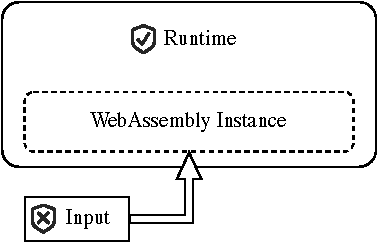
\includegraphics{figures/build/wasm-internal-mem-safety}
        \caption{Internal Memory Safety}
        \label{fig:internal-mem-safety}
    \end{subfigure}
    \hfill
    \begin{subfigure}[T]{0.45\textwidth}
        \centering
        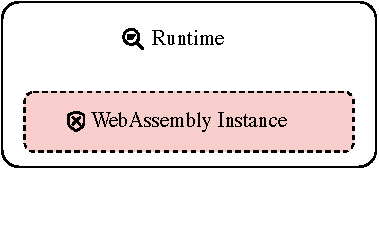
\includegraphics{figures/build/wasm-external-mem-safety}
        \caption{External Memory Safety}
        \label{fig:external-mem-safety}
    \end{subfigure}
    \caption{Threat model for internal and external memory safety}
    \label{fig:threat-model}
\end{figure}

\begin{description}
    \item[Internal Memory Safety]: Ensures memory safety within the boundaries of a sandbox.
    Our point of view is from within a WebAssembly instance, we trust the runtime (and the host we are running on), but we do not trust external input.
    See \cref{fig:internal-mem-safety}
    \item[External Memory Safety]: Maintains the memory safety of the sandbox itself against potentially malicious programs.
    Our point of view is from the runtime, we trust the platform we're running on, but not the WebAssembly programs we are executing.
    See \cref{fig:external-mem-safety}
\end{description}

\paragraph{Internal Memory Safety}
For internal memory safety, the program within the sandbox and its runtime are considered trusted.
Untrusted input (e.g., network data, file reads) originates from outside the sandbox.
This model mirrors the threat environment of a standard non-\ac{WASM} program.
Potential threats include:

\begin{description}
    \item[Buffer overflows] Attempts to write data beyond allocated buffer boundaries.
    \item[Use-after-free] Accessing memory after it has been deallocated.
\end{description}

WebAssembly's design inherently mitigates certain threats common in non-WASM environments, so we will not consider the following vectors:

\begin{description}
    \item[Return-oriented attacks] WASM's structured control flow constructs prevent arbitrary code execution through stack manipulation.
    \item[Calling unknown function pointers] Function tables enforce a strict mechanism for function calls, ensuring the integrity of call targets.
\end{description}

\paragraph{External Memory Safety}

For external memory safety, we focus on the security of the sandbox.
Threats originate from running untrusted programs, which may be buggy or adversarial.

\begin{itemize}
    \item \textbf{Sandbox escapes}: Attempts to break out of the sandbox's restrictions and access host resources.
    \item \textbf{Side-channel attacks}: Exploiting timing differences or resource usage patterns to infer sensitive information.
\end{itemize}


We assume that the runtime compiling and executing, as well as the operating system and underlying target architecture is free of bugs that might be exploited by malicious targets.
This includes assumptions that the WASM to native compilers inserts spectre guards where appropriate and properly manages bounds checks, e.g.\ by inserting appropriate guard pages.

% \projectname{} leverages the unique characteristic of WebAssembly's 64-bit pointers, which only use 48 bits for actual memory indexing.
% This design choice enables the efficient utilization of the remaining 16 bits for embedding metadata, such as tags or pointer signatures.
% Crucially, this approach does not necessitate any modifications to the code that operates on tagged addresses.

\begin{figure*}[t]
    \centering
    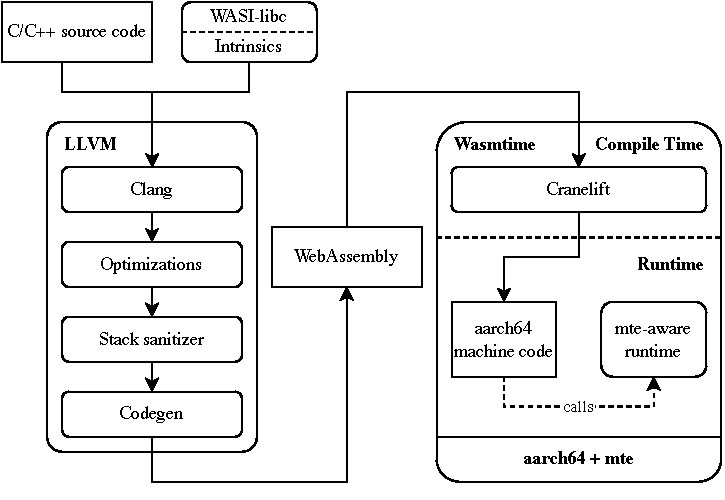
\includegraphics{figures/build/overview}
    \caption{Overview}
    \label{fig:overview}
\end{figure*}

\begin{figure}[t]
    \centering
    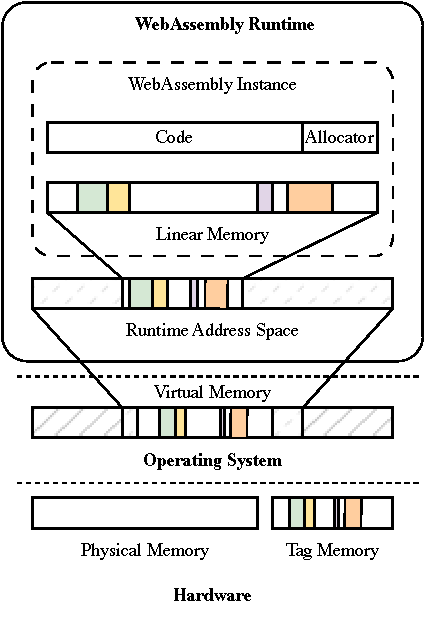
\includegraphics[scale=1]{figures/build/system-design-2}
    \caption{System Design of our Memory Safety Extension.}
    \label{fig:system-design-2}
\end{figure}

\begin{figure}[t]
    \centering
    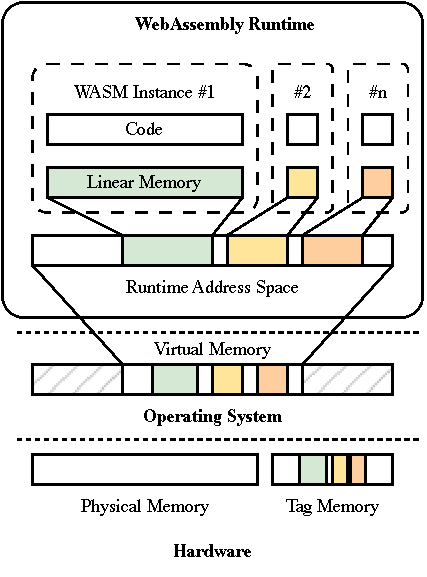
\includegraphics[scale=1]{figures/build/system-design-1}
    \caption{Bounds checks are replaced with MTE}
    \label{fig:system-design-1}
\end{figure}

Figure~\ref{fig:overview} presents an overview of \projectname{}.
In the WebAssembly context, a module contains one or more heaps, representing the linear memory accessible to the module.
Unlike programs compiled to native binaries, WebAssembly programs access memory through indices starting at zero, with zero being a valid address.
The runtime is responsible for setting up the linear memory at startup and translating indices to actual memory addresses by adding the heap base address to the index when accessing memory.
Crucially, the runtime is also required to perform bounds checks for memory accesses, which account for a large runtime overhead.

We build on top of \texttt{wasm64}, which allows indexing up to $2^{48}$ bytes, crucially leaving 16 unused bits in each address.
This aligns with most hardware implementations, which also just use 48 bits of an address to index into memory.

We reserve these bits to store metadata for each pointer.
Since WebAssembly does not have a dedicated pointer type, but uses plain integer types as pointers, these bytes can be manipulated using integer instructions.
We do, however, introduce three primitives in the form of new instructions to create and manipulate tagged memory regions, which also set the metadata tags in pointers.

\begin{itemize}
    \item \texttt{segment.new(i64, i64) $\rightarrow$ i64}: Allocates a new memory segment at the specified index and size, assigning it a randomly generated tag.
    \item \texttt{segment.set\_tag(i64, i64, i64)}: Applies a user-defined tag to the memory segment identified by the given index and size.
    \item \texttt{segment.free(i64, i64)}: Deallocates a memory segment, simultaneously re-tagging the corresponding index and size range to invalidate any pointers referencing this area.
\end{itemize}

The runtime environment raises a trap for any instruction that accesses memory segments with non-matching tags.

Existing instructions that access memory are inherently compatible with this system and do not require any modifications.
They are capable of handling both tagged and untagged indices.
This design choice allows the gradual integration of safety primitives into specific parts of WebAssembly applications where enhanced security is required.
For instance, it enables the introduction of a customized malloc implementation, which prevents spatial and temporal safety bugs for heap-allocated memory.

\todo{write about alignment}

The following C code will be used to demonstrate how the generated code will look like.

\begin{lstlisting}[frame=h,style=customc,
    label={code:wasm-example-c}]
char buf[64];
// ...
return;
\end{lstlisting}

\begin{lstlisting}[frame=h,style=customwasm,
    label={lst:wasm-example}]
;; Allocate space on the stack
global.get $__stack_pointer
i64.const 64
i64.sub
global.tee $__stack_pointer

;; tag the segment
i64.const 64
segment.new
local.set $buf

;; ...

;; retag with stack pointer tag
local.get $buf
global.get $__stack_pointer
i64.const 64
segment.set_tag

;; reset stack pointer
global.get $__stack_pointer
i64.const 64
i64.sub
global.set $__stack_pointer
\end{lstlisting}

\section{Heap Safety}

Heap safety is solved by aligning all allocations to 16 bytes and tagging the memory before returning to the caller.
When freeing memory, the freed memory is retagged to detect use-after-free errors.

\section{Stack Safety}

To achieve stack safety, we also tag stack allocations when entering a function and retag them when leaving a function.
However, tagging each stack slot is impractical due to significant performance and memory overheads.
The need to align each stack slot to the tag granularity adds to this issue, leading to excessive stack space consumption and elevated performance costs, particularly for stack slots that do not require this protection, such as slots for scalar variables.

To address this challenge, we propose an algorithm that identifies memory regions within the stack that do not require protection, thus avoiding tagging slots that do not contribute to stack safety. % rephrase
Our approach focuses on tagging only those stack slots that are indexed using indices that cannot be statically verified to remain within the slot's size.
Our analysis is not interprocedural to keep the algorithm simple.
Slots that have their address taken, thus escape our analysis and are also tagged.
Below we show a simplified version of our algorithm:

\begin{algorithmic}
    \State $allocsToInstrument \gets \emptyset$
    \For{$alloc \in allocations$}
        \If{escapes($alloc$)}
            \State $allocsToInstrument$.push($alloc$)
        \EndIf
        \If{isUsedByUnsafeGEP($alloc$)}
            \State $allocsToInstrument$.push($alloc$)
        \EndIf
    \EndFor

    \For{$alloc \in allocsToInstrument$}
        \State insertTaggingCode($alloc$)
        \State insertUntaggingCode($alloc$)
    \EndFor
\end{algorithmic}


In the code example below, \texttt{i} is safe, as it is not accessed using indices and its address does not escape.
The variables \texttt{bytes\_read} and \texttt{buf} are determined to be unsafe, as their address escapes.
Additionally, \texttt{buf} is accessed using an untrusted index, potentially leading to buffer overflows.

\begin{lstlisting}[frame=h,style=customc,
    label={code:stack-safety}]
char function(int index) {
  int i = 0; // safe
  int bytes_read = 0; // unsafe
  char buf[32]; // unsafe
  read_input(buf, &bytes_read);
  return buf[index];
}
\end{lstlisting}

\noindent
This method effectively balances the need for stack safety with performance and memory efficiency constraints.
Before returning, we ensure that all stack slots are untagged.
This provides temporal safety, preventing stack slots from being accessed after returning from a function.

\section{Bounds Checks}
\label{sec:bounds-checks}

WebAssembly runtimes ensure that applications remain within their allocated memory sandbox.
This is traditionally achieved through bounds checks or by leveraging the operating system's virtual memory management.
In wasm32, runtimes typically employ memory-mapping techniques, statically mapping the entire 32\,bit addressable space and marking unpermitted areas as inaccessible.
Accessing these inaccessible pages results in a segmentation fault, which is caught by the runtime, effectively containing the guest code within its sandbox.

However, this strategy faces limitations in wasm64 due to the impracticality of mapping the entire 64-bit address space.
This constraint necessitates the insertion of bounds checks, which can significantly degrade performance.
We demonstrate the impact of these checks on wasm64 execution speed in section~\ref{ch:eval}.

In \todo{ref:fig\_design\_bounds\_checks}, we showcase a approach that utilizes memory tagging to replace traditional bounds checks in wasm64 environments.
On module instantiation, the runtime assigns a predefined tag to the linear memory and the heap base address.
Memory access translation then involves adding this tagged heap base address to the accessed index.

\subsubsection{Combining memory safety with MTE bounds checks}

\begin{figure}[t]
    \centering
    %\begin{adjustbox}{max width=\textwidth}
    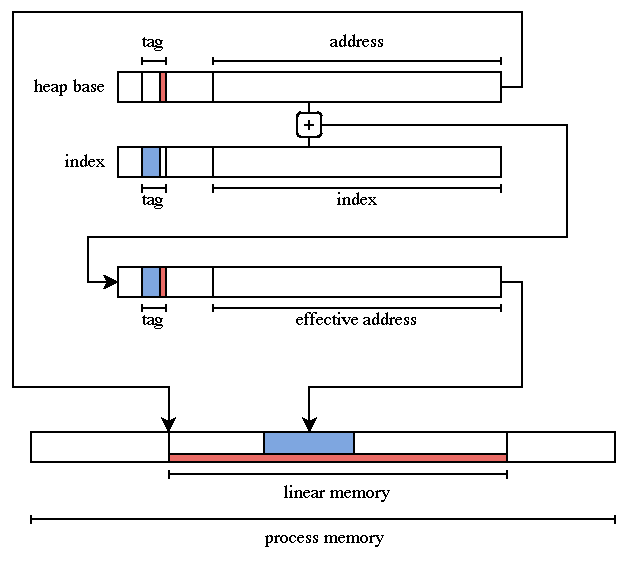
\includegraphics[scale=0.75]{figures/build/bounds-mem-safety}
    %\end{adjustbox}
    \caption{Bounds checks are replaced with MTE}
    \label{fig:system-design-mem-safety-bounds}
\end{figure}

To combine these two approaches, it is important to not allow users to escape from the sandbox by forging tags but still benefit from the
performance gained from removing bounds checks.

There is two challenges we need to take care of.
\begin{enumerate}
    \item Adding a tagged user pointer to the heap base address should be performant and result in the cprrect tag for the respective memory.
    \item It's crucial to prevent users from creating tags that enable access beyond their allocated memory sandbox.
\end{enumerate}

To circumvent these issues, designate the lowest tag bit to determine whether memory belongs to the runtime or to the linear memory.
Inaccessible memory us tagged with 0, while the linear memory is initially tagged with the tag 1.
The remaining three tag bits are used for the memory safety features and can be generated by \texttt{segment.new}.
When tagging memory using these primitives, we set the lowest tag bit to 1 before tagging.
Since the memory index is untrusted, an attacker may craft a value that overflows the tag bits when adding it to the heap base, resulting in a tag that allows accessing memory outside the linear memory.
To prevent this, we need to set the lowest tag bit via a bitwise mask before each memory access.
The code for this can be seen in listings~\ref{lst:generated-code-mem-access} and~\ref{lst:generated-code-mem-access}.

\begin{lstlisting}[frame=h,style=customc,
    label={lst:generated-code-tagging}]
// tagging memory
v0 = or tag, 0x0100_0000_0000_0000
stzg v0, [address]
\end{lstlisting}

\begin{lstlisting}[frame=h,style=customc,
    label={lst:generated-code-mem-access}]
// accessing memory
v0 = add heap_base, index
v1 = or v1, 0x0100_0000_0000_0000
\end{lstlisting}

With this approach, we prevent attempts by untrusted code to access runtime memory through forged tags.

